\section{Introduction}
Data are susceptible to various forms of corruption such as missing, incorrect, or inconsistent representations \cite{Gartner}.
Dirty data can lead to inaccurate analysis and cleaning data is a well studied problem \cite{rahm2000data}.
The growing popularity of predictive models (e.g., fraud detection) in data analytics \cite{bdas, alexandrov2014stratosphere, crotty2014tupleware, hellerstein2012madlib} adds additional challenges in managing dirty data.
Preditive models rely on learning relationships between features and labels, and systematic corruption \cite{taylor1982introduction}, where corruption disproportionately affects certain data, can introduce spurious relationships.
The high dimensionality of these models can amplify even a small amount of corruption \cite{xiaofeature}.
%Consequently, predictions from models trained on systematically corrupted data can be error-prone.

To make this problem concrete, consider a music recommender system in which due to a software bug, all users from Europe have an incorrect age attribute defaulted to ``18-24".
A recommendation model trained on this data may spuriously learn a correlation relationship between the ``18-24" age group and music liked by European users.
A bug, which ostensibly affected only the European users, now affects predictions to all users aged ``18-24".
Systematic corruption prior to featurization is not addressed in the robust Machine Learning literature which focuses on the resilience to outliers (i.e., age ``150").

A variety of data cleaning frameworks have been recently proposed \cite{khayyat2015bigdansing, chu2015katara, sampleclean} to address the problem of corrupted data.
However, data analysts report that data cleaning remains one of the most time consuming steps in the analysis process \cite{nytimes}.
Data cleaning can require a significant amount of developer effort in writing software or rules to fix the corruption.
Crowdsourcing is an increasingly popular alternative with recent success in missing value filling and entity resolution \cite{gokhale2014corleone, park2014crowdfill, sampleclean,chu2015katara}.
However, crowdsourcing comes at the cost of additional latency and the overhead of managing human workers.

Thus, for many corrupted datasets, \emph{progressive data cleaning} is important, where analysts can inspect early results with only $k \ll N$ records cleaned.
Early results allow analysts to judge the impact of an expensive or time consuming data cleaning operation without cleaning the entire data.
However, when applied with predictive modeling, progressive data cleaning poses three main methodological problems: mixing, sampling, and corruption sparsity.
Suppose $k$ records are cleaned, but all of the remaining dirty records are retained in the dataset.
Training a model on a mixture of dirty and clean data can lead to misleading relationships in even simple scenarios (Figure \ref{update-arch1}).
The alternative is to clean $k$ records and to disregard all of the remaining dirty records (e.g., \cite{wang1999sample}).
While this avoids the mixing problem, accurate model training can require a large amount of training data and $k$ examples may not be enough for a viable model.
Finally, both problems are compounded by sparsity, were if corrupted records are uncommon, random sampling of the $N$ total records may find relatively few examples of corruptions.
The errors introduced by these three problems may dominate any gains from data cleaning, leading to unreliable or misleading conclusions about data or model quality.

\begin{figure}[t]
\centering
 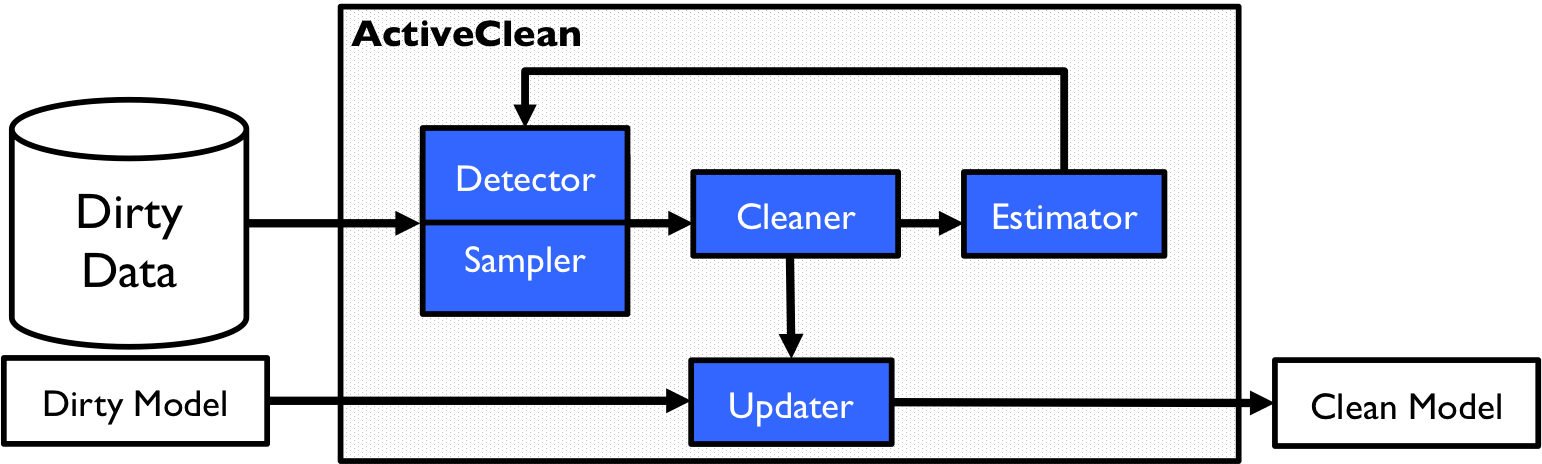
\includegraphics[width=\columnwidth]{figs/arch.png}
 \caption{\sysfull is an architecture where data cleaning is integrated with model training in a framework with sampling, model update, and feedback through estimation. \label{sys-arch}}\vspace{-2em}
\end{figure}

We propose \sys to address the progressive data cleaning problem in a way that avoids the three challenges: mixing, sampling, and sparsity.
The key insight is that an important class of predictive models, called convex-loss models (e.g., linear regression and SVMs), are trained by iteratively drawing random samples of data and updating a model\cite{bertsekas2011incremental}.
Data cleaning can be integrated with the sampling and updating training process; preserving provable guarantees such as convergence and error bounds.
Data are cleaned in small random batches and the model is incrementally updated based on the results.
Similar to Active Learning, \sys selects the most valuable records to clean with higher probability, however, it applies a number of optimizations that exploit the data cleaning setting such as avoiding data that is expected to be clean, estimating of the effect of data cleaning for a record, and batching together updates from already cleaned data.

The \sys architecture (Figure \ref{sys-arch}) consists of a \emph{detector}, \emph{sampler}, \emph{cleaner}, \emph{updater}, and \emph{estimator}.
The cleaner is an existing data cleaning framework (e.g., Entity Resolution), and \sys provides the remaining components to apply this framework progressively.
To summarize the contributions in each component:
\begin{itemize}[noitemsep]
\item Detector (Section \ref{det}). The detector can apply rules from data quality constraints or adaptively learn which records are dirty to increase the fraction of dirty records sampled.
\item Sampler (Section \ref{dist-samp}). We derive an optimal sampling distribution that minimizes the update variance (i.e., how different would the update be if we drew another sample) which linearly improves an error bound on the convergence rate.
\item Updater (Section \ref{model-update}). The updater applies a weighted stochastic gradient descent step to the current best model. This update converges if all of the data is cleaned, and for batch size $b$ and iterations $T$, converges with rate $O(\frac{1}{\sqrt{bT}})$. 
\item Estimator (Section \ref{sampling}) The estimator applies a Taylor Series linearization to decouple changes in different features using knowledge about what is wrong with the data to better estimate the impact of an error.
\item We evaluate these components on 4 datasets with real and synthetic corruption (Section \ref{eval}). For a 5\%  systematic corruption, to achieve the same accuracy as a state-of-the-art Active Learning algorithm cleaning 1000 records, \sys cleans 55\% less records on average.
\end{itemize}






